\chapter{A review on quaternion algebra and its Fourier transform}
\label{ch:reviewQuat}

In 1833, at the age of 28, Willian Rowan Hamilton presented to the Royal Irish Academy (RIA) a work in which complex numbers were treated as ordered pairs of real numbers, given the appropriate definition of operations.\footnote{The results were published in 1837, in the paper \emph{Theory of Conjugate Functions, or Algebraic Couples; with a Preliminary and Elementary Essay on Algebra as the Science of Pure Time} \cite{hamilton1837theory}.} In the following years, he struggled to extend the complex field into a normed division algebra over triples, but soon realized that, as much as his attempts were inventive, the resulting algebra\footnote{An \textit{algebra over a field}, or simply \textit{algebra}, is a vector space over a field with a bilinear multiplication (that is, the multiplication distributes over the addition and the associativity is valid for multiplication) \cite{schafer1955introduction}.} was not closed under multiplication. We can see this through a simple example \cite{santos2011algebra}: let it be the set $\mathbb{F} = \{ a + b \qi + c \qj  \ | \ (a, b, c) \in \mathbb{R}^3\}$, with $\qi^2 = \qj^2 = -1$ and $\qi \neq \qj$. Since $\qi, \qj \in \mathbb{F}$, so there should exist $x, y, z \in \mathbb{R}$ so that
\begin{equation}
    \qi \qj = x + y \qi + z \qj.
    \label{eq:demonstration01}
\end{equation}

Multiplying by $\qi$ both sides of the equation,
\begin{equation}
    \qi^2 \qj = \qi x + \qi^2 y + z (\qi \qj),
\end{equation}
and using (\ref{eq:demonstration01}) it yields,
\begin{equation}
    - \qj = \qi x - y + z (x + y \qi + z \qj)
    \iff
    (zx - y) + \qi (x + zy) + \qj (z^2 + 1) = 0.
\end{equation}
That is: $z \notin \mathbb{R}$ and $ \qi \qj \notin \mathbb{F} $, proving that such algebraic structure is not closed under multiplication.

Only a decade later, in 1843, while walking by the roads in Dublin toward the RIA, ``an electric circuit seemed to close, and a spark flashed forth,'' as he would say. He had conceived the four-dimensional structure required to the desired algebra, creating the quaternions. Moved by excitement, he craved on the stone below Broome Bridge, in Cabra (Dublin), the equations that define the relations between the canonical basis elements of quaternions.\footnote{Close to the original site of the inscriptions, the RIA placed a commemorative plaque in 1958, with the same writings.} This creation, made possible by an insight in 1843, is found accross most of this work. The following sections lead the reader through the foundations of quaternion algebra and quaternion signal analysis.


\section{Introduction to the quaternion algebra}

Quaternions are numbers $q \in \mathbb{H}$ in the form
\begin{equation}
    q = a + b\qi + c\qj + d\qk,
    \label{eq:q}
\end{equation}
in which $a, b, c, d \in \mathbb{R}$, holding true the fundamental relations:
\begin{equation}
    \label{eq:fund_rel}
    \begin{aligned}
        \qi ^2 = \qj^2 & =\qk^2 = \qi \qj \qk = -1.
    \end{aligned}
\end{equation}

The multiplication rules between  $ \qi $, $ \qj $ and $ \qk $ follow directly from (\ref{eq:fund_rel}), resembling those between orthonormal basis vectors from $ \mathbb{R}^3 $ and the vector product: the product between two of them yields the third, the sign being determined from the operands order. For instance, to find the result of $ \qi \qj $ one may start from (\ref{eq:fund_rel}) and write
\begin{equation}
    \begin{aligned}
        \qi \qj \qk                         & = -1   \\
        \qi \qj \underbrace{\qk \qk}_{= -1} & = -\qk \\
        \qi \qj                             & = \qk.
    \end{aligned}
\end{equation}
Similarly, to find $ \qj \qi $,
\begin{equation}
    \begin{aligned}
        \qi \qj \qk     & = -1        \\
        \qi \qi \qj \qk & = -\qi      \\
        - \qj \qk       & = - \qi     \\
        \qj \qj \qk     & =  \qj \qi  \\
        - \qk           & =  \qj \qi. \\
    \end{aligned}
\end{equation}
Fig. \ref{fig:quatmult} depicts the order in which the product between any pair in the triplet $ \qi $, $ \qj $ and $ \qk $ yields the third one, with positive sign. All three units commute with real numbers. The most relevant consequence, therefore, of (\ref{eq:fund_rel}), is that the quaternion product is \textit{noncommutative}. In fact, it is the first example of noncommutative normed division algebra in history \cite{kleiner2007history}.

\begin{figure}
    \centering
    \caption{Illustration of the multiplication rule between the imaginary units $ \qi $, $ \qj $ and $ \qk $.}
    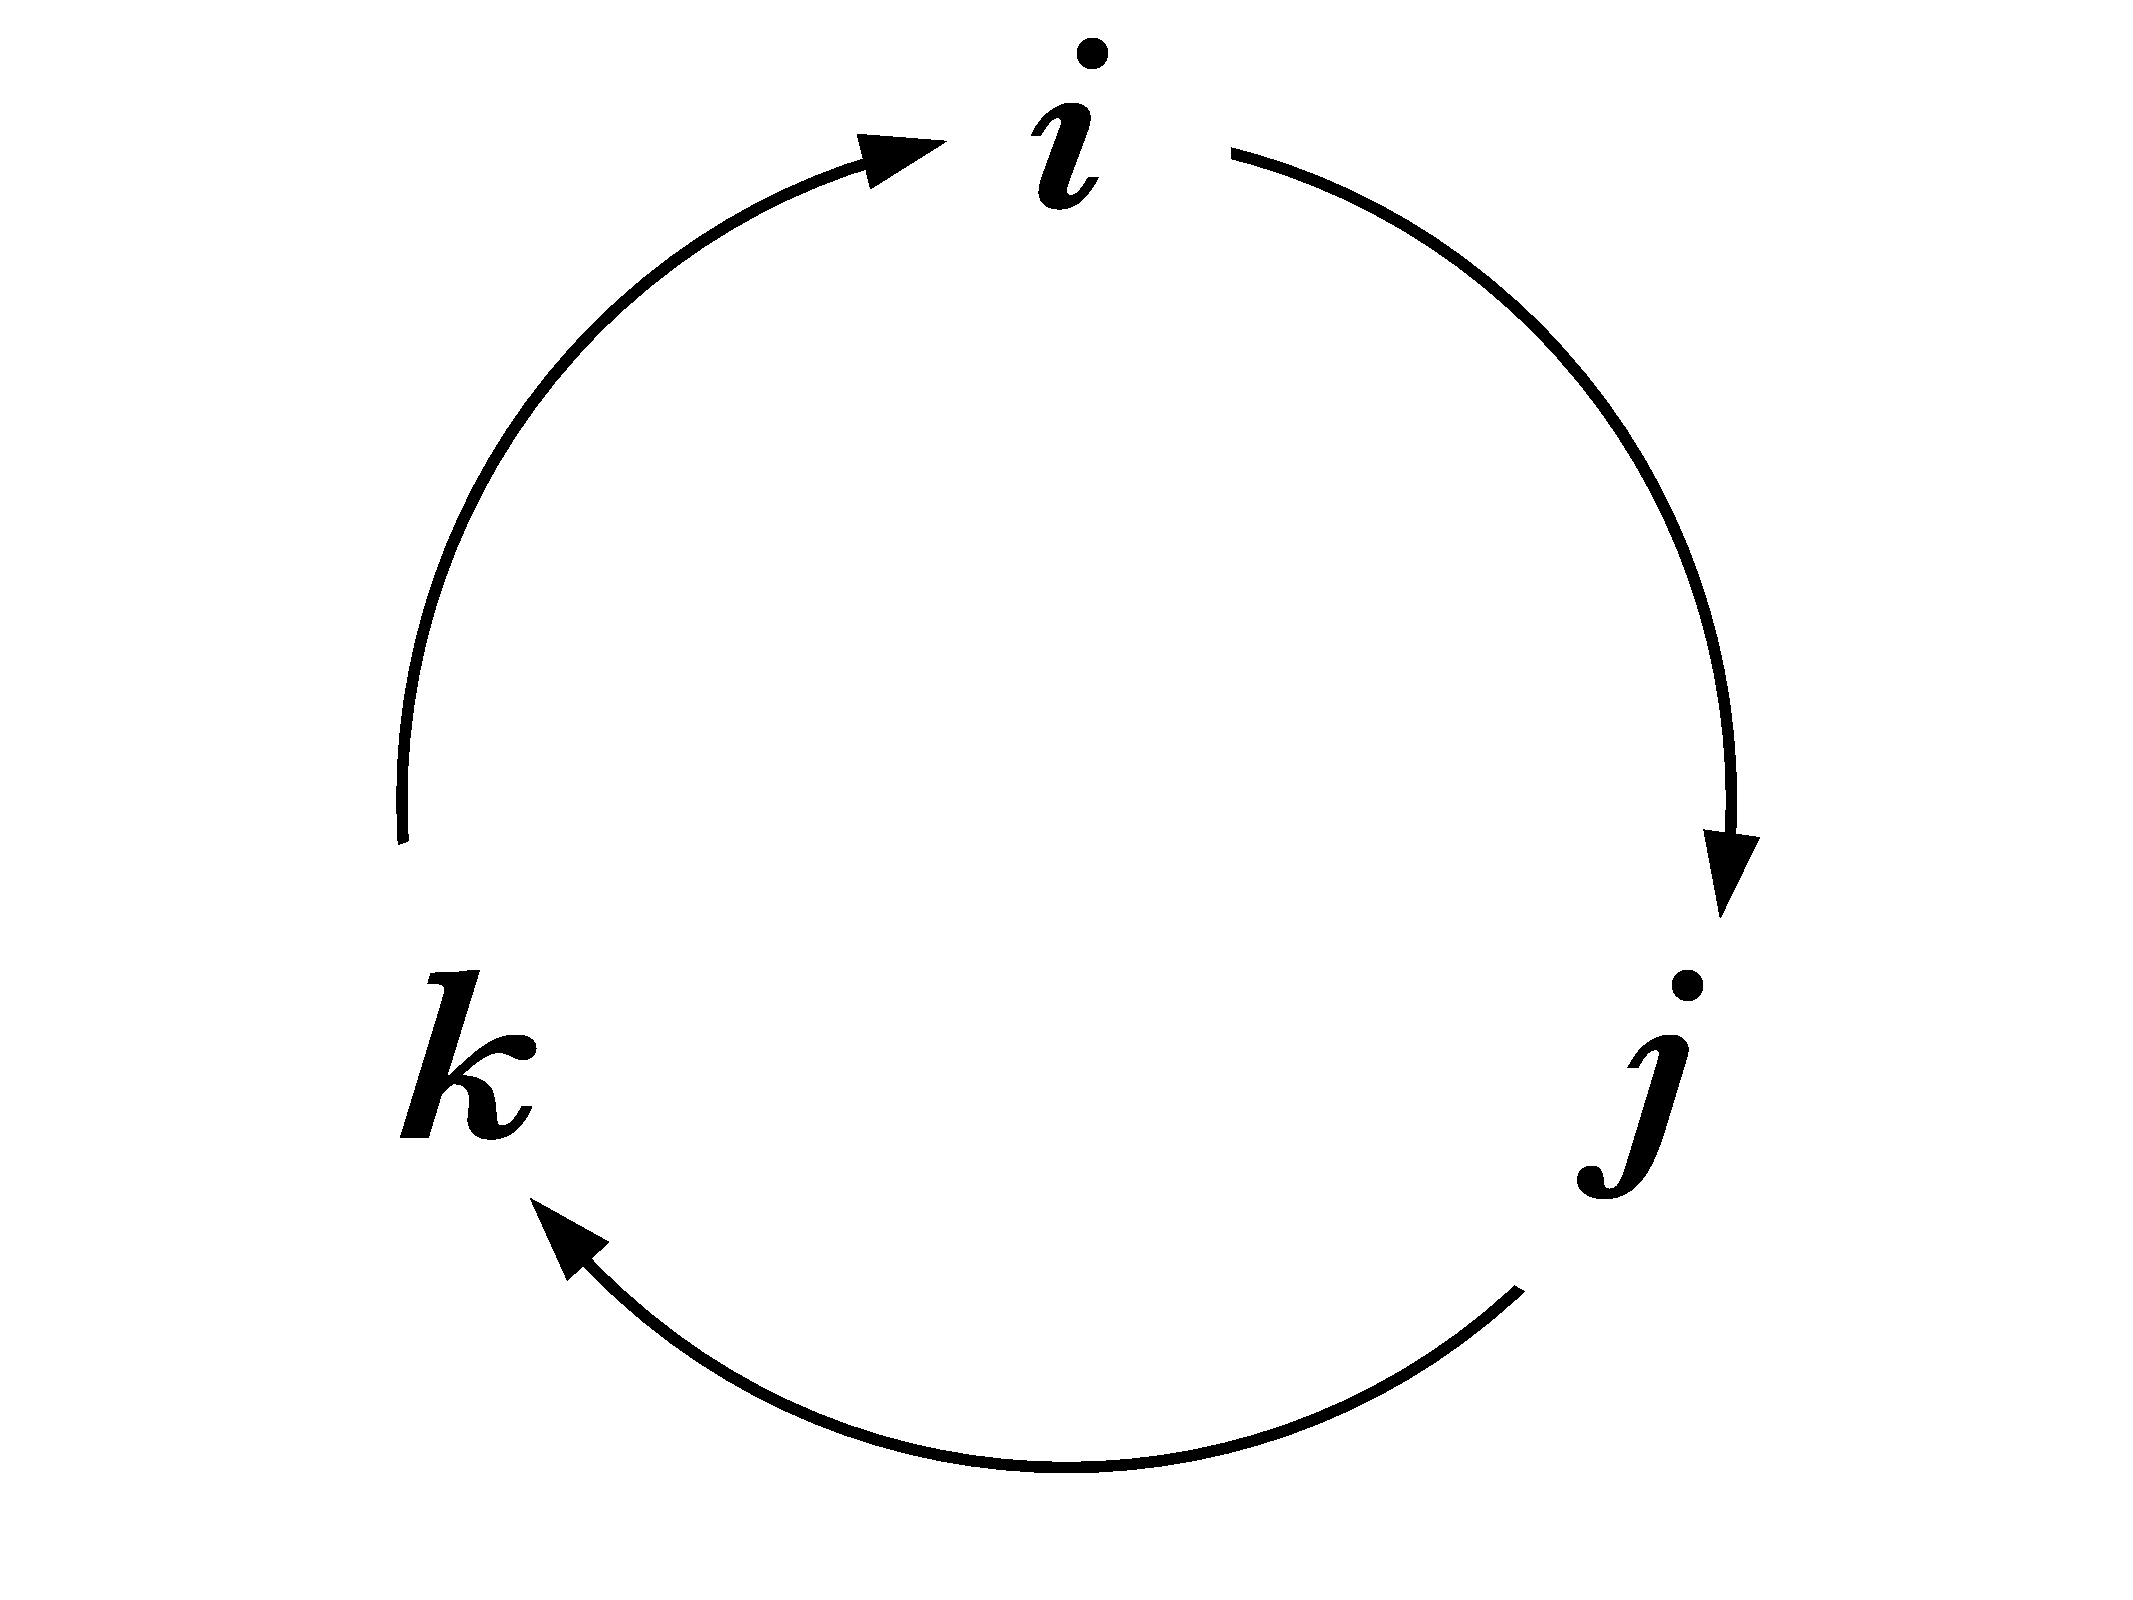
\includegraphics[width=0.2\linewidth]{Figures/quaternion_multiplication.pdf}
    \floatsource
    \label{fig:quatmult}
\end{figure}